
\section{Fibonacci Hexagon}
Once $F$-matrices are defined for a TQFT, consistency of the $R$-matrix is enforced by the so-called hexagon equations as shown in the figure diagramatically by Fig. 13.11. or the Fibonacci anyon theory, once the $F$-matrix is fixed as in Eq. 9.3, the $R$-matrices are defined up to complex conjugation (i.e., there is a right and left handed Fibonacci anyon theory - both are consistent). Derive these $R$-matrices. Confirm Eqs. 10.2 as one of the two solutions and show no other solutions exist.

\paragraph{Answer}


\section{Evaluation of a Diagram}
Consider the following diagram:
\begin{figure}[h!]
\centering
\tikzset{every picture/.style={line width=0.75pt}} %set default line width to 0.75pt        

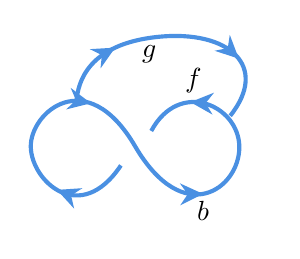
\begin{tikzpicture}[x=0.75pt,y=0.75pt,yscale=-1,xscale=1]
%uncomment if require: \path (0,101); %set diagram left start at 0, and has height of 101

%Curve Lines [id:da820170391940162] 
\draw [color={rgb, 255:red, 74; green, 144; blue, 226 }  ,draw opacity=1 ][line width=1.5]    (321.41,67.3) .. controls (301.9,96.57) and (278.49,75.1) .. (278,58.52) .. controls (277.51,41.93) and (304.83,18.03) .. (328.24,58.03) .. controls (351.65,98.03) and (378.48,78.52) .. (378.48,58.52) .. controls (378.48,38.52) and (349.7,25.35) .. (336.04,50.71) ;
\draw [shift={(290.61,79.09)}, rotate = 21.86] [fill={rgb, 255:red, 74; green, 144; blue, 226 }  ,fill opacity=1 ][line width=0.08]  [draw opacity=0] (11.07,-5.32) -- (0,0) -- (11.07,5.32) -- (7.35,0) -- cycle    ;
\draw [shift={(306.97,37.36)}, rotate = 191.69] [fill={rgb, 255:red, 74; green, 144; blue, 226 }  ,fill opacity=1 ][line width=0.08]  [draw opacity=0] (11.07,-5.32) -- (0,0) -- (11.07,5.32) -- (7.35,0) -- cycle    ;
\draw [shift={(360.97,81.02)}, rotate = 178.91] [fill={rgb, 255:red, 74; green, 144; blue, 226 }  ,fill opacity=1 ][line width=0.08]  [draw opacity=0] (11.07,-5.32) -- (0,0) -- (11.07,5.32) -- (7.35,0) -- cycle    ;
\draw [shift={(354.91,36.8)}, rotate = 3.87] [fill={rgb, 255:red, 74; green, 144; blue, 226 }  ,fill opacity=1 ][line width=0.08]  [draw opacity=0] (11.07,-5.32) -- (0,0) -- (11.07,5.32) -- (7.35,0) -- cycle    ;
%Curve Lines [id:da5627695777560877] 
\draw [color={rgb, 255:red, 74; green, 144; blue, 226 }  ,draw opacity=1 ][line width=1.5]    (300.07,36.12) .. controls (300.7,27.63) and (305.31,8.77) .. (339.46,5.35) .. controls (373.6,1.94) and (393.11,19.5) .. (374.09,43.4) ;
\draw [shift={(318.68,10.55)}, rotate = 150.88] [fill={rgb, 255:red, 74; green, 144; blue, 226 }  ,fill opacity=1 ][line width=0.08]  [draw opacity=0] (11.07,-5.32) -- (0,0) -- (11.07,5.32) -- (7.35,0) -- cycle    ;
\draw [shift={(378.21,15.86)}, rotate = 223.7] [fill={rgb, 255:red, 74; green, 144; blue, 226 }  ,fill opacity=1 ][line width=0.08]  [draw opacity=0] (11.07,-5.32) -- (0,0) -- (11.07,5.32) -- (7.35,0) -- cycle    ;

% Text Node
\draw (356.61,83.17) node [anchor=north west][inner sep=0.75pt]    {$b$};
% Text Node
\draw (350.85,19) node [anchor=north west][inner sep=0.75pt]    {$f$};
% Text Node
\draw (330.11,8) node [anchor=north west][inner sep=0.75pt]    {$g$};
\end{tikzpicture}
\end{figure}
Evaluate this diagram in terms of $R$'s and $F$'s. Hint: First reduce the diagram to that shown in exercise 12.1.

\paragraph{Answer}

\section{Gauge transform of $R$ and Hexagon}

\begin{enumerate}
\item Confirm the gauge transform Eq. 13.3.
\item Show that a set of $F$-matrices and $R$-matrices satisfying the hexagon equations, Eq. 13.1 and 13.2 remains a solution after a gauge transformation. Remember that both $R$ - and $F$-transform.
\end{enumerate}

\paragraph{Answer}

\section{Reidermeister Moves}

\begin{enumerate}
\item Use the $R$-matrix, and the completeness relationship, to derive the equivalence shown on the left of Fig. 13.9.
\item How does the hexagon equation imply the equivalence shown in Fig.\ref{fig:ReidermeisterMoveAndRMatrix}. Hint: This is very subtle, but is almost trivial.
\item Use Fig.\ref{fig:ReidermeisterMoveAndRMatrix} to show the equality on the right of Fig. 13.9.
\item Use the result of Fig. 13.14 along with completeness and the $R$-matrix to demonstrate Fig. 13.10.
\end{enumerate}

\begin{figure}[h!]
\centering
\tikzset{every picture/.style={line width=0.75pt}} %set default line width to 0.75pt        

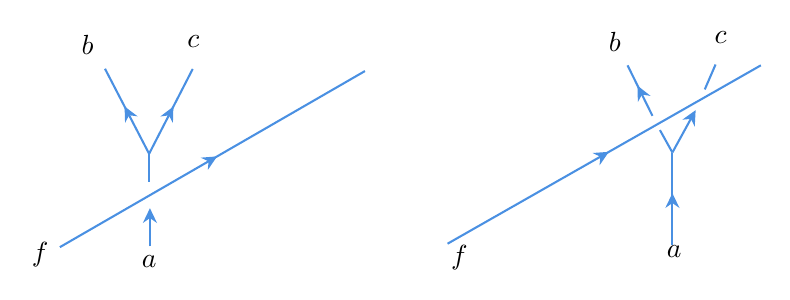
\begin{tikzpicture}[x=0.75pt,y=0.75pt,yscale=-1,xscale=1]
%uncomment if require: \path (0,121); %set diagram left start at 0, and has height of 121

%Straight Lines [id:da08398462617264979] 
\draw [color={rgb, 255:red, 74; green, 144; blue, 226 }  ,draw opacity=1 ]   (169,105.24) -- (316.01,20.39) ;
\draw [shift={(244.75,61.52)}, rotate = 150.01] [fill={rgb, 255:red, 74; green, 144; blue, 226 }  ,fill opacity=1 ][line width=0.08]  [draw opacity=0] (7.14,-3.43) -- (0,0) -- (7.14,3.43) -- (4.74,0) -- cycle    ;
%Straight Lines [id:da37507964086028056] 
\draw [color={rgb, 255:red, 74; green, 144; blue, 226 }  ,draw opacity=1 ]   (212,60.24) -- (233.01,19.39) ;
\draw [shift={(223.69,37.51)}, rotate = 117.21] [fill={rgb, 255:red, 74; green, 144; blue, 226 }  ,fill opacity=1 ][line width=0.08]  [draw opacity=0] (7.14,-3.43) -- (0,0) -- (7.14,3.43) -- (4.74,0) -- cycle    ;
%Straight Lines [id:da1021191401550543] 
\draw [color={rgb, 255:red, 74; green, 144; blue, 226 }  ,draw opacity=1 ]   (212,60.24) -- (190.75,19.28) ;
\draw [shift={(200.18,37.46)}, rotate = 62.58] [fill={rgb, 255:red, 74; green, 144; blue, 226 }  ,fill opacity=1 ][line width=0.08]  [draw opacity=0] (7.14,-3.43) -- (0,0) -- (7.14,3.43) -- (4.74,0) -- cycle    ;
%Straight Lines [id:da9646759688994204] 
\draw [color={rgb, 255:red, 74; green, 144; blue, 226 }  ,draw opacity=1 ]   (212,73.68) -- (212,60.24) ;
%Straight Lines [id:da24803612552618537] 
\draw [color={rgb, 255:red, 74; green, 144; blue, 226 }  ,draw opacity=1 ]   (212.4,104.88) -- (212.4,89.48) ;
\draw [shift={(212.4,86.48)}, rotate = 90] [fill={rgb, 255:red, 74; green, 144; blue, 226 }  ,fill opacity=1 ][line width=0.08]  [draw opacity=0] (7.14,-3.43) -- (0,0) -- (7.14,3.43) -- (4.74,0) -- cycle    ;

%Straight Lines [id:da2734825019858991] 
\draw [color={rgb, 255:red, 74; green, 144; blue, 226 }  ,draw opacity=1 ]   (355.8,103.57) -- (506.74,17.64) ;
\draw [shift={(433.53,59.32)}, rotate = 150.35] [fill={rgb, 255:red, 74; green, 144; blue, 226 }  ,fill opacity=1 ][line width=0.08]  [draw opacity=0] (7.14,-3.43) -- (0,0) -- (7.14,3.43) -- (4.74,0) -- cycle    ;
%Straight Lines [id:da8145882952858203] 
\draw [color={rgb, 255:red, 74; green, 144; blue, 226 }  ,draw opacity=1 ]   (464.12,104.04) -- (464.12,59.64) ;
\draw [shift={(464.12,79.24)}, rotate = 90] [fill={rgb, 255:red, 74; green, 144; blue, 226 }  ,fill opacity=1 ][line width=0.08]  [draw opacity=0] (7.14,-3.43) -- (0,0) -- (7.14,3.43) -- (4.74,0) -- cycle    ;
%Straight Lines [id:da027527400071296615] 
\draw [color={rgb, 255:red, 74; green, 144; blue, 226 }  ,draw opacity=1 ]   (464.12,59.64) -- (473.87,41.87) ;
\draw [shift={(475.32,39.24)}, rotate = 118.77] [fill={rgb, 255:red, 74; green, 144; blue, 226 }  ,fill opacity=1 ][line width=0.08]  [draw opacity=0] (7.14,-3.43) -- (0,0) -- (7.14,3.43) -- (4.74,0) -- cycle    ;
%Straight Lines [id:da1340583515504703] 
\draw [color={rgb, 255:red, 74; green, 144; blue, 226 }  ,draw opacity=1 ]   (479.72,29.24) -- (484.92,17.24) ;
%Straight Lines [id:da7371201039902171] 
\draw [color={rgb, 255:red, 74; green, 144; blue, 226 }  ,draw opacity=1 ]   (464.12,59.64) -- (458.12,48.84) ;
%Straight Lines [id:da178128564489902] 
\draw [color={rgb, 255:red, 74; green, 144; blue, 226 }  ,draw opacity=1 ]   (454.52,41.97) -- (442.52,17.64) ;
\draw [shift={(447.37,27.47)}, rotate = 63.74] [fill={rgb, 255:red, 74; green, 144; blue, 226 }  ,fill opacity=1 ][line width=0.08]  [draw opacity=0] (7.14,-3.43) -- (0,0) -- (7.14,3.43) -- (4.74,0) -- cycle    ;


% Text Node
\draw (154,101.24) node [anchor=north west][inner sep=0.75pt]    {$f$};
% Text Node
\draw (207,108) node [anchor=north west][inner sep=0.75pt]    {$a$};
% Text Node
\draw (178,1.74) node [anchor=north west][inner sep=0.75pt]    {$b$};
% Text Node
\draw (229,1.74) node [anchor=north west][inner sep=0.75pt]    {$c$};
% Text Node
\draw (432,-0.01) node [anchor=north west][inner sep=0.75pt]    {$b$};
% Text Node
\draw (483,-0.01) node [anchor=north west][inner sep=0.75pt]    {$c$};
% Text Node
\draw (356,103) node [anchor=north west][inner sep=0.75pt]    {$f$};
% Text Node
\draw (460,103) node [anchor=north west][inner sep=0.75pt]    {$a$};
\end{tikzpicture}
\caption{This move is implied by the hexagon equation. (Similar with the straight line $f$ going under the other two, and similar if the left-to-right slope of $f$ is negative instead of positive.).}
\label{fig:ReidermeisterMoveAndRMatrix}
\end{figure}

This exercise shows that equalities like those shown in Fig. 13.9 and 13.10 are not independent assumptions but can be derived from the planar algebra and the definition of an $R$-matrix satisfying the hexagon.
